%
% Tesi D.S.I. - modello preso da
% Stanford University PhD thesis style -- modifications to the report style
%
%%%%%%%%%%%%%%%%%%%%%%%%%%%%%%%%%%%%%%%%%%%%%%%%%%%%%%%%%%%%%%%%%%%%%%%%%%%
%                                                                         %
%			TESI DOTTORATO                                                   %
%			______________                                                   %
%                                                                         %
%			AUTORE: Elena Pagani                                             %
%                                                                         %
%			Ultima revisione: 7.X.1998                                       %
%           correzioni atrent                                             %
%%%%%%%%%%%%%%%%%%%%%%%%%%%%%%%%%%%%%%%%%%%%%%%%%%%%%%%%%%%%%%%%%%%%%%%%%%%
%
%
\begin{filecontents*}[overwrite]{\jobname.xmpdata}
\Title{UTILIZZO DI SERVIZI BASATI SULLA POSIZIONE IN UN'APPLICAZIONE DI MONITORAGGIO DELLE PRESENZE}
\Author{Simone Paolo Petta}
\Language{it-IT}
\Subject{Tesi di informatica per la comunicazione digitale.}
\Keywords{Tesi}
\end{filecontents*}
\documentclass[a4paper,12pt]{report}
%    \renewcommand{\baselinestretch}{1.6}      % interline spacing
%
% \includeonly{}
%
%			PREAMBOLO
%

\usepackage[a4paper]{geometry}
\usepackage{amssymb,amsmath,amsthm}
\usepackage{graphicx}
\usepackage{subcaption}
\usepackage{hyperref}
\usepackage{xcolor}
\usepackage{epsfig}
\usepackage[italian]{babel}
\usepackage{setspace}
\usepackage{tesi}
\usepackage{listings}
\usepackage{pgfplots}
\usepackage{xurl}
\usepackage{colorprofiles}
\usepackage[a-1a,mathxmp]{pdfx}[2018/12/22]
\hypersetup{pdfstartview=} 

\hypersetup{
    colorlinks=true,
    linkcolor=black,
    linkbordercolor=white,
    urlcolor=black, % Colore dei link URL (cambia a seconda delle tue preferenze)
    citecolor=black % Colore dei link alle citazioni (cambia a seconda delle tue preferenze)
}

% per le accentate
\usepackage[utf8]{inputenc}
%
\newtheorem{myteor}{Teorema}[section]
%
\newenvironment{teor}{\begin{myteor}\sl}{\end{myteor}}
%
%
%			TITOLO
%
\begin{document}
\title{UTILIZZO DI SERVIZI BASATI SULLA POSIZIONE IN UN'APPLICAZIONE DI MONITORAGGIO DELLE PRESENZE}
\author{Simone Paolo PETTA}
\dept{Corso di Laurea in informatica per la comunicazione digitale} 
\anno{2022-2023}
\relatore{Prof. Sergio MASCETTI}
\correlatore{Silvia GALUZZI}
%
%        \submitdate{month year in which submitted to GPO}
%		- date LaTeX'd if omitted
%	\copyrightyear{year degree conferred (next year if submitted in Dec.)}
%		- year LaTeX'd (or next year, in December) if omitted
%	\copyrighttrue or \copyrightfalse
%		- produce or don't produce a copyright page (false by default)
%	\figurespagetrue or \figurespagefalse
%		- produce or don't produce a List of Figures page
%		  (false by default)
%	\tablespagetrue or \tablespagefalse
%		- produce or don't produce a List of Tables page
%		  (false by default)
% 
%			DEDICA
%
\beforepreface
% \prefacesection{}
%         {\hfill \Large {\sl DEDICHE}}
% % 
% %			PREFAZIONE
% %
% \prefacesection{Prefazione}
% hkjafgyruet.
% %
% %
% %			ORGANIZZAZIONE
% \section*{Organizzazione della tesi}
% \label{organizzazione}
% La tesi \`e organizzata come segue:
% \begin{itemize}
% \item nel Capitolo 1 ....
% \end{itemize}
%
%			RINGRAZIAMENTI
%
\prefacesection{Ringraziamenti}
Vorrei dedicare questo spazio a tutte le persone che, in modi diversi, hanno contribuito a rendere possibile il completamento del mio percorso accademico.

\medskip

Innanzitutto, desidero esprimere la mia profonda gratitudine alla mia famiglia. Il loro sostegno costante, la pazienza e l'amore hanno reso possibile questa esperienza accademica. Grazie per essere sempre stati al mio fianco e per avermi sostenuto nei momenti di difficoltà.

\medskip

Un ringraziamento speciale va ai miei amici, che hanno condiviso con me gioie e sfide durante questi anni. Le vostre risate, il vostro supporto e la vostra amicizia hanno reso ogni passo di questo viaggio più significativo.

\medskip

Un sentito ringraziamento va anche a tutte le persone che, anche solo con una parola di incoraggiamento, hanno contribuito a spingermi avanti nei momenti più difficili.

\medskip

Infine, desidero ringraziare me stesso per la dedizione e il duro lavoro che ho messo in questo percorso accademico. Questa tesi è il risultato del mio impegno e della mia passione. Sono grato di aver avuto l'opportunità di affrontare questo viaggio.

\medskip

Grazie a tutti coloro che hanno reso questo percorso un'esperienza indimenticabile.

\afterpreface
% 
% 
%			CAPITOLO 1: dshjkfg
\chapter{Introduzione}
\label{cap1}
%
%
L'azienda Zucchetti S.P.A., tramite delle web application, fornisce numerosi servizi per la gestione del personale, tra i quali sono presenti servizi per la gestione delle paghe, di selezione e formazione delle risorse umane e di monitoraggio delle presenze. L'insieme di queste web application prende il nome di suite HR (Human Resources) di Zucchetti S.P.A.. La suite HR è resa disponibile anche su dispositivi mobili, tramite l'applicazione ZConnect, che attualmente conta un ampio bacino di utenti, con circa 720.000 utenti Android e circa 120.000 utenti iOS. La versione Android di ZConnect è sviluppata in Java e Kotlin, mentre per l'ambiente iOS è stato utilizzato Swift.

Tra i numerosi servizi offerti da ZConnect, uno di particolare importanza per questo lavoro è quello di monitoraggio delle presenze. Tale servizio permette all'utente di registrare la propria presenza sul luogo di lavoro utilizzando il dispositivo mobile personale. L'utente ha quindi la possibilità di recarsi sul posto di lavoro ed una volta entrato nell'area geografica che identifica il luogo preposto per registrare la propria presenza, può effettuare la timbratura.
Il lavoratore si può quindi trovare in due situazioni: all'interno dell'area di timbratura o all'esterno. Se si trova all'interno, ZConnect permette all'utente di registrare la propria presenza sul luogo di lavoro e di visualizzare una mappa, sulla quale è rappresentata l'area di lavoro tramite la funzionalità del geofence, il quale rappresenta un perimetro virtuale attorno a un luogo specifico \cite{GeoFence}. Se invece si trova all'esterno, il lavoratore non ha la possibilità di registrare la propria presenza sul luogo di lavoro, ma può visualizzare una mappa sulla quale è rappresentata solamente la sua posizione tramite un marker.

Zucchetti S.P.A. fornisce ZConnect ad un'azienda cliente, che per motivi di riservatezza non è possibile citare, che quindi verrà indicata come Azienda X. La collaborazione con Azienda X ha fatto emergere delle limitazioni del servizio di monitoraggio delle presenze di ZConnect.
La complessa configurazione delle aree di lavoro dell'Azienda X, che spesso si estendono su ampie porzioni del territorio, ha presentato una serie di sfide significative per i dipendenti nell'utilizzo del servizio di monitoraggio delle presenze di ZConnect. In queste aree non sono presenti edifici o strutture fisiche facilmente raggiungibili, i dipendenti quindi non hanno punti di riferimento chiari in cui registrare la loro presenza.
Questo scenario ha reso complesso per i dipendenti l'accesso alle aree di lavoro designate per la timbratura. La mancanza di edifici o riferimenti facilmente identificabili ha creato un notevole disagio, poiché gli utenti si sono trovati a dover navigare in ambienti geografici sconosciuti, spesso estesi e non facilmente riconoscibili.
Inoltre, l'applicazione ZConnect non era in grado di fornire un feedback adeguato per guidare i dipendenti verso le aree di timbratura, poiché mancava un elemento fondamentale, una mappa navigabile che mostrasse chiaramente la posizione dell'utente e identificasse l'area di lavoro più vicina. Questa mancanza di un quadro visivo completo non agevolava i dipendenti nel raggiungimento delle aree di registrazione della presenza creando in loro frustrazione nell'utilizzo di questa funzionalità.

L'obiettivo di questo lavoro di tesi è quello di risolvere le limitazioni del sistema di monitoraggio delle presenze indicate dall'Azienda X. Per risolvere queste limitazioni è stata modificata la visualizzazione ed il comportamento della mappa di ZConnect.
\'E stata modificata la visualizzazione della mappa in modo da include la posizione dell'utente e l'area di timbratura più vicina, rappresentata tramite la funzionalità del geofence. Questo risultato è stato reso possibile grazie all'implementazione di una funzionalità di zoom della mappa. Quando l'utente apre la mappa, una porzione della mappa è automaticamente ingrandita e centrata sulla sua posizione attuale, che è rappresentata da un marker. Contemporaneamente, l'area di timbratura più vicina, delimitata dal geofence, è chiaramente visibile sulla mappa. Questo approccio garantisce che l'utente possa vedere la propria posizione e l'obiettivo da raggiungere immediatamente all'apertura della mappa, semplificando il processo di navigazione.
Per agevolare il raggiungimento dell'area di timbratura è stato reso il marker che rappresenta la posizione dell'utente dinamico, facendolo muovere seguendo gli spostamenti del device dell'utente, in modo tale che il lavoratore veda in tempo reale, consultando la mappa, la direzione in cui si sta spostando. Avendo questo riscontro visivo immediato per il lavoratore risulta più semplice raggiungere l'area di registrazione delle presenze anche in ambienti a lui non familiari e privi di punti di riferimento.
\'E  stata anche implementata una funzionalità di ``follow-me" che rende più agevole l'utilizzo della mappa.
La funzionalità di ``follow-me" è stata progettata per semplificare l'esperienza dell'utente durante lo spostamento. Grazie a questa funzionalità, il lavoratore non è più costretto a interagire continuamente con la mappa durante il proprio spostamento per dover vedere la propria posizione. Invece, la mappa viene resa dinamica e gestisce automaticamente l'area visualizzata a schermo.
Con la funzionalità ``follow-me" attiva, la mappa segue in tempo reale il movimento dell'utente, garantendo che la propria posizione sia sempre al centro della porzione di mappa visualizzata.

Il processo di sviluppo del miglioramento della funzionalità di monitoraggio delle presenze ha comportato un attento lavoro di analisi, progettazione, sviluppo e test, al fine di garantire un prodotto finale affidabile e soddisfacente.
Per sviluppare questa funzionalità, mi sono unito al team di sviluppo e manutenzione di ZConnect, composto da 11 membri. Questo team è responsabile sia dello sviluppo Android che iOS. All'interno del gruppo, ho svolto l'analisi, la progettazione e lo sviluppo della funzionalità, lavorando su entrambe le piattaforme Android e iOS. Ho scritto il codice in modo indipendente e successivamente è stato oggetto di revisione da parte di alcuni colleghi del team di sviluppo. Dopo la fase di sviluppo, ho collaborato con il team di testing, diverso rispetto al team di sviluppo e manutenzione di ZConnect, per condurre una serie di test funzionali sulla nuova versione di ZConnect prodotta con questo lavoro di tesi.
Superati i test tecnici la funzionalità è stata ufficialmente rilasciata nell'applicazione ZConnect, resa disponibile agli utenti sia su piattaforma Android che iOS. Attualmente la funzionalità è utilizzata da centinaia di migliaia di persone.
Questo approccio ha garantito che il prodotto fosse pienamente funzionante, testato e pronto per l'utilizzo su larga scala.

\chapter{Analisi}
\label{cap2}

Il presente lavoro di tesi ha l'obiettivo di migliorare il sistema di monitoraggio delle presenze dell'applicazione ZConnect di Zucchetti S.P.A.. Inizialmente è stata affrontata una fase di analisi per poter comprendere chi avrebbe utilizzato il sistema di monitoraggio delle presenze, qual'era lo stato attuale del sistema, nella versione Android e iOS, e per capire quali requisiti doveva soddisfare l'implementazione, come descritto nelle Sezioni 2.1, 2.2 e 2.3 di questo capitolo.

Durante l'analisi, è stata posta particolare attenzione a garantire un supporto di facile e immediata consultazione per gli utenti, soprattutto per agevolare la registrazione della presenza nel luogo designato. L'analisi ha contribuito a identificare gli obiettivi principali del nuovo sistema, nonché i requisiti funzionali e non funzionali che dovevano essere soddisfatti.

L'obiettivo di questo capitolo è presentare in dettaglio i risultati dell'analisi condotta, evidenziando le sfide affrontate, le conclusioni tratte e come tali risultati hanno orientato l'implementazione del sistema di monitoraggio delle presenze in azienda basato sulla geolocalizzazione.

\section{Analisi degli attori}

Gli utenti che utilizzeranno la funzionalità per registrare le proprie presenze in azienda sono i dipendenti dell'azienda a cui è venduta l'applicazione ZConnect, in particolar modo i dipendenti dell'Azienda X. I dipendenti dell'azienda X che utilizzeranno questa funzionalità sono in maggior parte degli operai edili che operano in aree di lavoro molto estese sul territorio. Ogni dipendente avrà accesso all'applicazione tramite un account personale, che gli consentirà di effettuare le operazioni di timbratura, utilizzando una mappa come supporto nel raggiungimento dell'area di lavoro, sarà inoltre possibile per gli utenti consultare il proprio storico delle presenze.

Gli utenti, quindi, hanno la necessità di utilizzare questa funzionalità in modo immediato, per poter registrare la propria presenza in azienda ed iniziare il loro lavoro. Hanno, inoltre, la necessità di poter consultare una mappa dinamica in cui siano facilmente identificabili la propria posizione e l'area in cui poter registrare la propria presenza più vicina a loro.

\section{Analisi del sistema esistente}\label{Analisi_sistema}

Come già menzionato nell'Introduzione l'applicazione ZConnect è sviluppata sia per Android \cite{Android}, utilizzando Java \cite{Java} e Kotlin \cite{Kotlin}, che per iOS \cite{iOS}, utilizzando Swift \cite{Swift}. Questo duplice sviluppo comporta delle differenze di implementazione, in quanto la stessa applicazione viene sviluppata per due sistemi operativi differenti utilizzando linguaggi differenti.

In entrambe le versioni di ZConnect per realizzare il servizio di monitoraggio delle presenze, a ciascun utente viene associata una lista di luoghi geografici all'interno dei quali è abilitato a registrare la propria presenza. Questi luoghi sono modellati come geofence, che rappresentano un perimetro virtuale attorno a un luogo specifico \cite{GeoFence}. L'associazione tra utente e luoghi geografici è effettuata dal server, all'applicazione viene inviata la lista dei luoghi associata all'utente.

All'interno dell'applicazione, un geofence è modellato attraverso un'interfaccia chiamata IGeoFence. L'interfaccia IGeoFence è identica sia nell'ambito di Android che di iOS. Questa interfaccia specifica il tipo di geofence, che può essere poligonale, circolare, quadrato, o anche di tipo nullo. Quest'ultima opzione è stata introdotta per modellare i tag NFC utilizzati in altre sezioni dell'applicazione, assimilandoli a geofence. L'interfaccia IGeoFence include anche una serie di metodi ``get" per recuperare informazioni come il tipo di geofence, il centro del geofence e le coordinate geografiche. In particolare, risultano fondamentali la latitudine e la longitudine massima e minima, poiché, nei casi d'uso attuali, tutti i geofence sono di tipo quadrato. Avendo a disposizione le latitudini e le longitudini minime e massime, è possibile delineare il perimetro dello spazio geografico modellato tramite il geofence con quattro punti.

Tramite un algoritmo, ZConnect verifica che la posizione dell'utente sia all'interno del perimetro di uno dei geofence associati all'utente. ZConnect esegue questo algoritmo quando l'utente è sulla schermata in cui può effettuare una timbratura ogni volta che rileva un cambio di posizione del device.
Gli utenti si possono trovare in due situazioni, all'esterno di un'area geografica preposta per la registrazione della presenza ed all'interno di un'area geografica preposta per la registrazione della presenza. Se si trovano all'interno di un'area geografica proposta per la registrazione della presenza, potranno effettuare la timbratura. Se invece si trovano all'esterno non potranno effettuare la registrazione della presenza.
In entrambi i casi, per gli utenti è possibile aprire una mappa. Nel caso in cui l'utente si trovi all'interno di un area in cui effettuare la timbratura, l'applicazione mostra il geofence indicato come valido per la timbratura centrando la mappa sul centro del geofence, con un marker, rosso per entrambe le versioni dell'applicazione, al centro dello stesso per indicare la posizione. Invece, nel caso in cui l'utente si trovi fuori da un'area in cui può effettuare la timbratura, l'applicazione mostra la mappa centrata sulla posizione dell'utente con un marker, rosso per la versione Android e blu per la versione iOS, che indicava la posizione dell'utente.

\begin{figure}[ht!]
    \begin{subfigure}{0.4\textwidth}
        \centering
        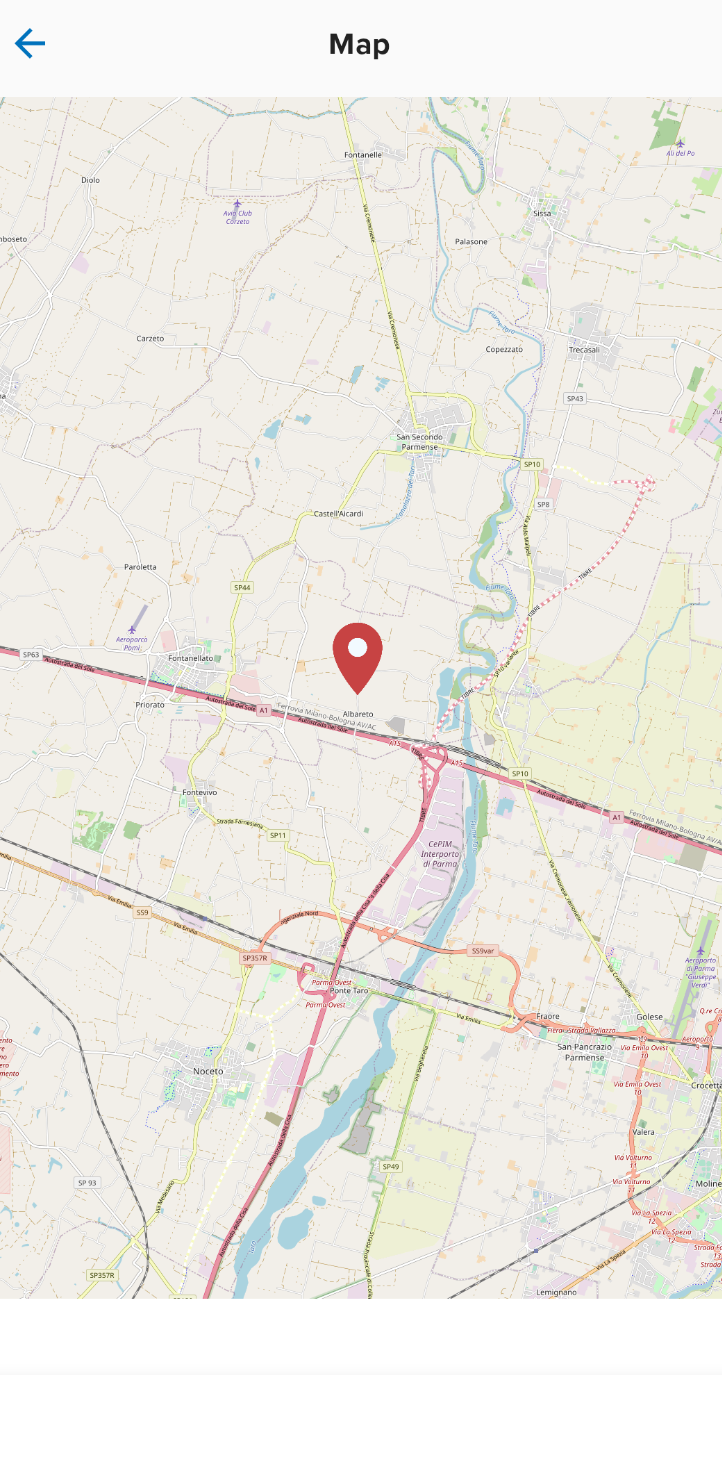
\includegraphics[width=\linewidth]{Immagini/vecchia_posizione_esterna.png}
        \caption{Mappa visualizzata quando l'utente è all'esterno di un geofence}
        \label{fig:vecchia_posizione_esterna_Android}
    \end{subfigure}
    \hspace{1cm} % Spazio orizzontale tra le immagini
    \begin{subfigure}{0.4\textwidth}
        \centering
        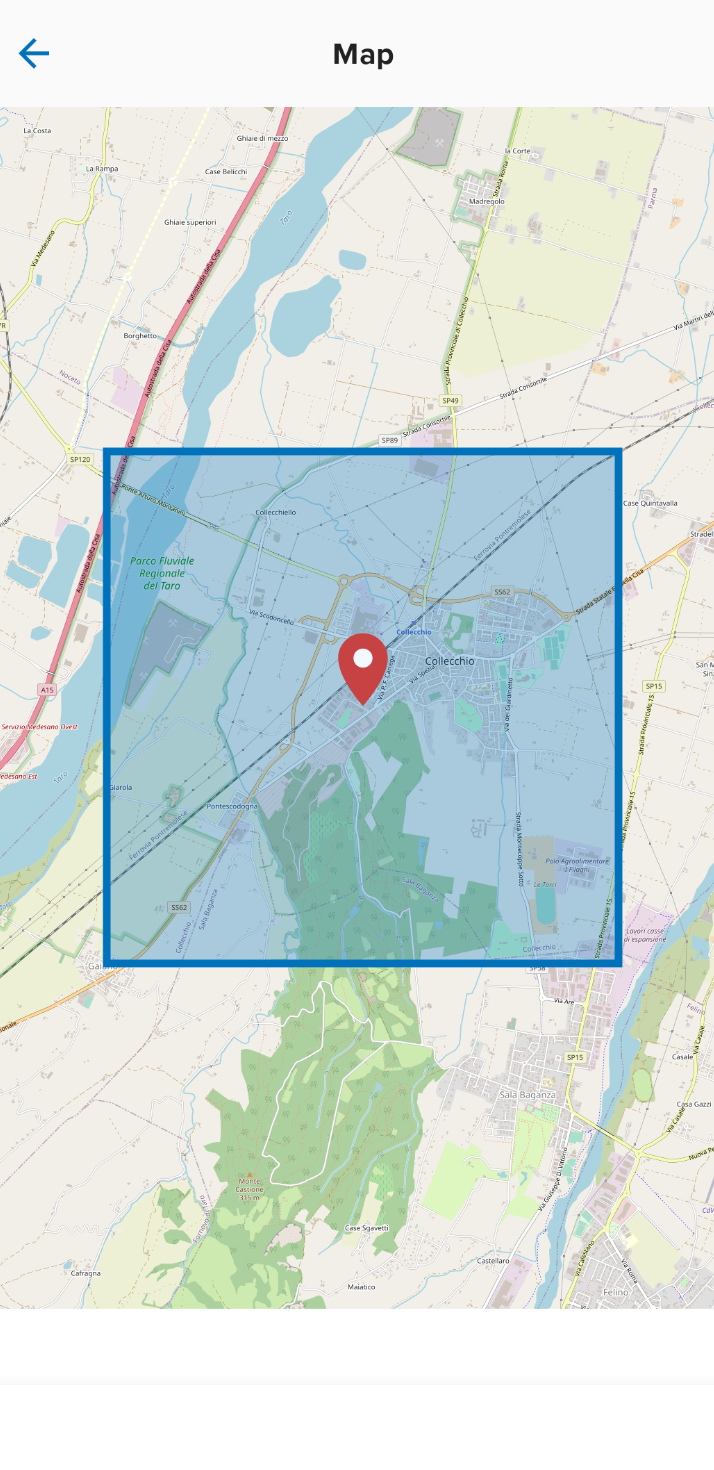
\includegraphics[width=\linewidth]{Immagini/vecchia_posizione_interna.png}
        \caption{Mappa visualizzata quando l'utente è all'interno di un geofence}
        \label{fig:vecchia_posizione_interna_Android}
    \end{subfigure}
    \caption{Mappa di ZConnect per Android}
    \label{fig:vecchia_mappa_android}
\end{figure}

\begin{figure}[ht!]
    \begin{subfigure}{0.4\textwidth}
        \centering
        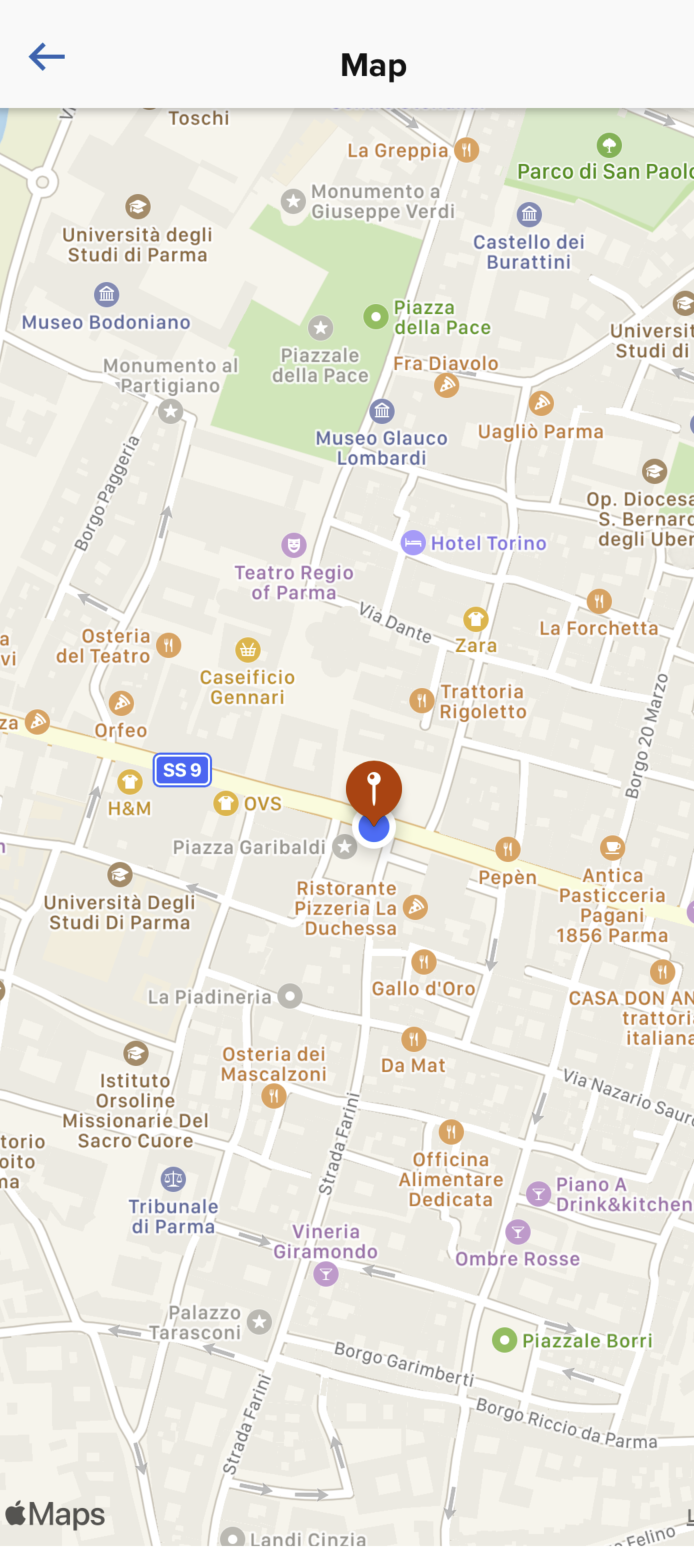
\includegraphics[width=\linewidth]{Immagini/vecchia_posizione_esterna_ios.png}
        \caption{Mappa visualizzata quando l'utente è all'esterno di un geofence}
        \label{fig:vecchia_posizione_esterna_iOS}
    \end{subfigure}
    \hspace{1cm} % Spazio orizzontale tra le immagini
    \begin{subfigure}{0.4\textwidth}
        \centering
        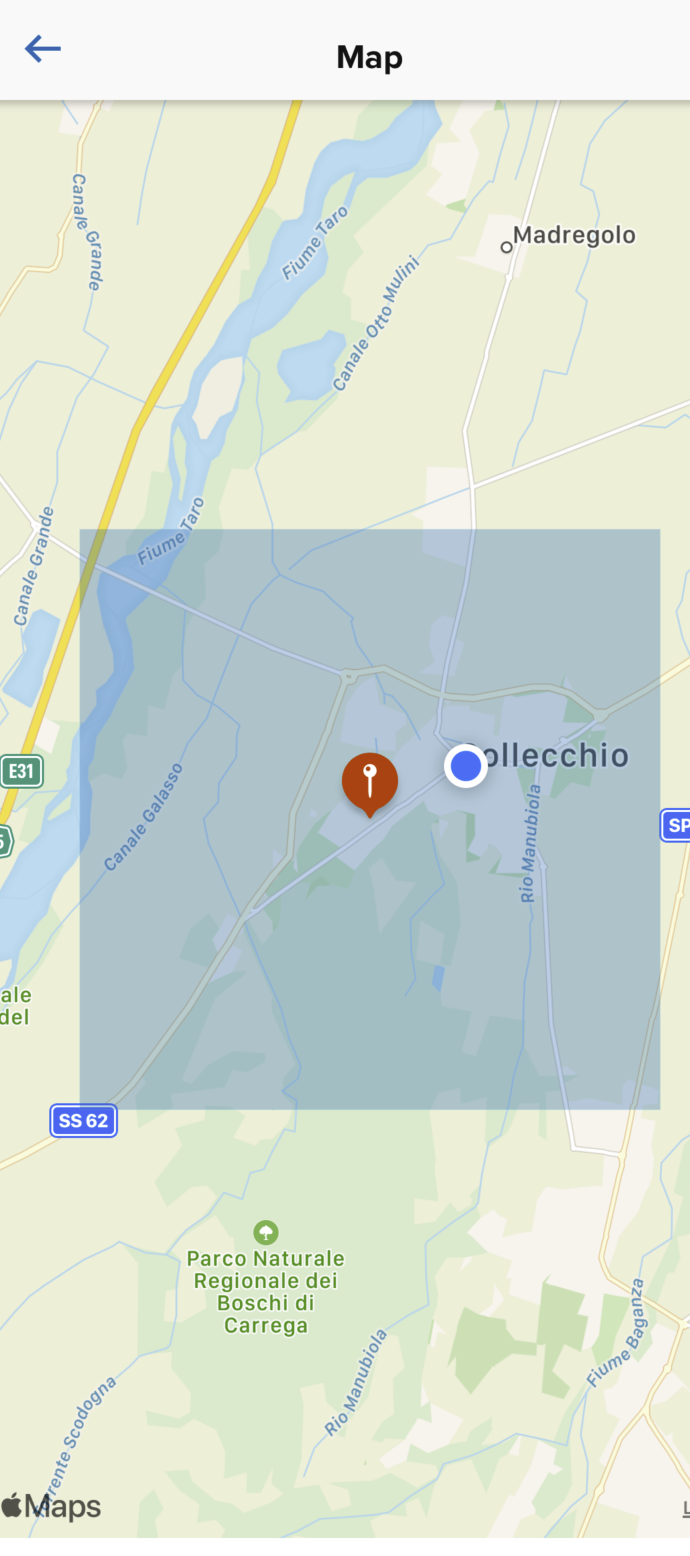
\includegraphics[width=\linewidth]{Immagini/vecchia_posizione_interna_ios.png}
        \caption{Mappa visualizzata quando l'utente è all'interno di un geofence}
        \label{fig:vecchia_posizione_interna_iOS}
    \end{subfigure}
    \caption{Mappa di ZConnect per iOS}
    \label{fig:vecchia_mappa_android_2}
\end{figure}

A causa del duplice sviluppo di ZConnect, l'implementazione delle mappe varia tra le due versioni.
Nella versione Android di ZConnect, viene utilizzata la libreria Osmdroid. Osmdroid è una libreria specifica per Android che offre strumenti per interagire con OpenStreetMap (OSM). OpenStreetMap (OSM) è un progetto collaborativo finalizzato a creare mappe del mondo a contenuto libero. Il progetto punta ad una raccolta mondiale di dati geografici, con scopo principale la creazione di mappe e cartografie \cite{OpenStreetMapWiki}.
Nel codice Android di ZConnect il fragment \cite{Fragment} che si occupa di mostrare la mappa è HRMapsOsmFragment. La mappa però nel fragment non viene gestita direttamente utilizzando i metodi forniti della libreria Osmdroid, ma viene utilizzata un'interfaccia IMapBinder, e la sua implementazione concreta OSMapBinder, che hanno lo scopo di esporre metodi per la gestione della mappa. L'interfaccia IMapBinder è stata progettata per poter garantire flessibilità per il futuro, in quanto è solamente l'implementazione concreta di IMapBinder ad utilizzare i metodi forniti dalla libreria delle mappe, rendendo così possibile cambiare la libreria in futuro senza dover modificare il codice dei fragment che mostrano la mappa.

Nella versione iOS di ZConnect, la visualizzazione della mappa è gestita utilizzando la libreria MapKit \cite{MapKitDoc}. La libreria MapKit è fornita direttamente da Apple e offre diverse funzionalità per l'integrazione delle mappe nelle applicazioni iOS.
A differenza di quanto fatto in Android, i metodi forniti dalla libreria MapKit vengono utilizzati direttamente nel ViewController \cite{ViewController} dedicato alla visualizzazione e all'interazione con la mappa, HRMapViewController. Alcuni dei metodi forniti dalla libreria MapKit permettono di impostare la regione di visualizzazione della mappa, aggiungere e personalizzare le annotazioni che rappresentano i luoghi di timbratura, e gestire le azioni dell'utente come lo zoom e lo spostamento sulla mappa.

\section{Problemi del sistema esistente}\label{Problemi_sistema}

Nell'implementazione precedente a questo lavoro di tesi del servizio di monitoraggio delle presenze di ZConnect, non veniva fornito un supporto adeguato agli utenti nel raggiungimento dell'area di lavoro, poiché, nel caso in cui l'utente si fosse trovato all'esterno di un'area di lavoro, la mappa non avrebbe mostrato con chiarezza la posizione dell'utente e la posizione dell'area di lavoro, fornendo un supporto inadeguato all'utente nel raggiungimento dell'area di lavoro, come è possibile vedere in Figura \ref{fig:vecchia_posizione_esterna_Android} e in Figura \ref{fig:vecchia_posizione_esterna_iOS}.

Questo limite creava una potenziale difficoltà per gli utenti nell'individuare con precisione l'area in cui dovevano registrare la propria presenza. L'assenza dei geofence sulla mappa impediva agli utenti di avere una visualizzazione diretta delle aree geografiche consentite per la timbratura, creando delle difficoltà nel raggiungimento del luogo di lavoro.

\section{Analisi dei requisiti}
La modifica del sistema di monitoraggio delle presenze, eseguita in questo lavoro di tesi, è stata guidata dalla necessità di soddisfare requisiti fondamentali. Il sistema rinnovato deve garantire all'utente la possibilità di registrare la propria presenza sul luogo di lavoro una volta raggiunto. Inoltre, l'utente deve avere la possibilità, sia che si trovi all'esterno di un luogo di lavoro, sia quando è all'interno, di visualizzare una mappa sulla quale sono rappresentati la propria posizione e tutti i luoghi di lavoro a lui associati, modellati come geofence. All'apertura della mappa, deve essere garantito un livello di zoom adeguato affinché l'utente possa visualizzare immediatamente la sua posizione e quella del luogo di lavoro più vicino.

Il marker che identifica la posizione dell'utente sulla mappa deve muoversi in tempo reale, seguendo gli spostamenti del dispositivo dell'utente, fornendo un feedback visivo immediato sulla direzione del movimento. Deve inoltre essere implementata una funzionalità "Follow-Me" che renda la mappa dinamica, garantendo che la posizione dell'utente sia sempre al centro della porzione di mappa visualizzata durante gli spostamenti.

\section{Analisi delle necessità}
La modifica del sistema di monitoraggio delle presenze deve essere progettata tenendo conto dell'utilizzo in movimento da parte degli utenti, pertanto richiede una connessione Internet per poter scaricare e visualizzare la mappa. Inoltre, è necessaria una connessione GPS per ricevere gli aggiornamenti di posizione e calcolare correttamente se il dispositivo si trova all'interno di un geofence abilitato per la timbratura o meno. È essenziale gestire accuratamente i casi in cui manca la connessione Internet o non è disponibile il segnale GPS.

Nel caso in cui il segnale GPS sia assente, il sistema deve essere in grado di gestire tale situazione. È importante fornire all'utente un feedback chiaro e tempestivo sullo stato della connessione GPS. Ad esempio, il sistema potrebbe visualizzare un messaggio di avviso o utilizzare indicazioni visive per comunicare che la posizione potrebbe non essere accuratamente rilevata.

Il sistema deve gestire in modo adeguato i casi in cui l'utente revoca o non concede i permessi per la localizzazione. In tali situazioni, è necessario fornire un'interfaccia chiara che guidi l'utente a concedere i permessi richiesti e spieghi l'importanza di tali autorizzazioni per il corretto funzionamento del sistema di monitoraggio delle presenze.

La corretta gestione delle connessioni Internet, del segnale GPS e dei permessi per la localizzazione è essenziale per garantire un'esperienza utente senza problemi e per consentire al sistema di funzionare in modo affidabile e preciso in diverse condizioni. Pertanto, è fondamentale che il sistema sia attentamente progettato e implementato per gestire efficacemente queste situazioni, garantendo una corretta registrazione delle timbrature e fornendo feedback adeguati all'utente durante l'utilizzo dell'applicazione.

Un'altra casistica fondamentale che il sistema deve gestire è quella relativa alla prevenzione di possibili falsificazioni della posizione del dispositivo da parte dell'utente. È fondamentale evitare che l'utente possa manipolare in qualsiasi modo la posizione registrata dal device, poiché ciò potrebbe consentire di registrare la propria presenza anche quando non si è fisicamente presenti sul posto di lavoro.
Prendere le dovute precauzioni per prevenire la falsificazione della posizione è essenziale per mantenere l'accuratezza e l'affidabilità del sistema di monitoraggio delle presenze.

\chapter{Progettazione}
\label{cap3}

La progettazione dell'interfaccia grafica e dell'esperienza utente (UX) è una fase cruciale nella realizzazione di un software di successo. Nel contesto dell'obiettivo di questa tesi, che mira a facilitare i dipendenti dell'Azienda X nel raggiungimento dei loro luoghi di lavoro, questa Sezione descrive le scelte di progettazione che hanno contribuito a creare un'interfaccia utente più intuitiva, attraverso un'esperienza di utilizzo migliorata della mappa di ZConnect.

La progettazione dell'interfaccia grafica e dell'UX è stata guidata dalla necessità di fornire ai dipendenti un accesso rapido e intuitivo alle informazioni necessarie per raggiungere i loro luoghi di lavoro e registrare le presenze. L'ottimizzazione di funzionalità chiave, come la visualizzazione della posizione corrente dell'utente e dei luoghi di lavoro associati, nonché l'introduzione di nuove caratteristiche, come il "follow-me", hanno contribuito in modo significativo al raggiungimento di questi obiettivi.

\section{Progettazione delle interfacce grafiche e della UX}\label{Progettazione}
La progettazione dell'interfaccia grafica e dell'esperienza utente (UX) costituisce un elemento significativo all'interno di questo lavoro di tesi. L'obiettivo fondamentale di questa fase è stato progettare sistemi in grado di agevolare i dipendenti dell'Azienda X nel raggiungimento dei luoghi di lavoro. Per conseguire tale scopo, è stato necessario rivisitare l'interfaccia grafica dell'applicazione ZConnect.

Come riportato nella Sezione \ref{Problemi_sistema} nell'implementazione precedente a questo lavoro di tesi, il servizio di monitoraggio delle presenze di ZConnect non forniva un supporto adeguato agli utenti nel raggiungimento dell'area di lavoro. Per risolvere questo problema, è stata progettata la mappa in modo che mostri chiaramente la posizione dell'utente e l'area di lavoro da raggiungere.

Inoltre, come riportato nella Sezione \ref{Analisi_sistema} del capitolo di Analisi, ad ogni utente di ZConnect è associata una lista di luoghi geografici, modellati come geofence, in cui l'utente può effettuare la timbratura. Data questa molteplicità di luoghi in cui l'utente può registrare la propria presenza, è stato progettato di visualizzarli tutti sulla mappa, contrariamente a quanto avveniva prima dell'intervento descritto in questa tesi, come visibile in Figura \ref{fig:tanti_geofence}. In modo tale da agevolare l'utente nel raggiungimento del luogo di lavoro corretto, infatti essendo associati all'utente numerosi luoghi geografici non è possibile sapere a priori quale è quello in cui l'utente deve recarsi, di conseguenza non è plausibile scegliere un solo luogo da mostrare all'utente sulla mappa, scartando gli altri.

\begin{figure}[ht!]
    \centering
    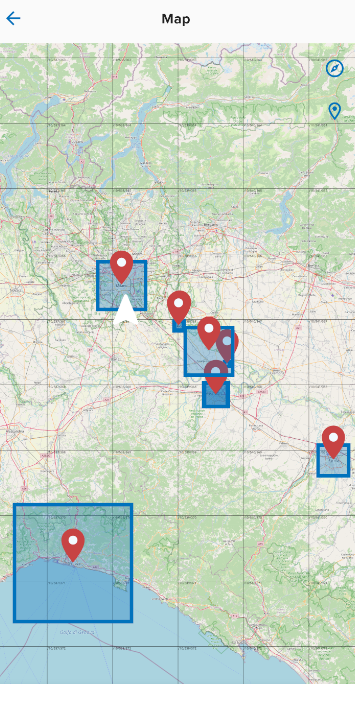
\includegraphics[width=0.4\textwidth]{Immagini/tanti_geofence.png}
    \caption{Mappa di un utente con tanti geofence}
    \label{fig:tanti_geofence}
\end{figure}

Al fine di garantire un'esperienza utente ottimale, è stato ritenuto essenziale rendere chiaramente visibili all'utente, all'apertura della mappa, la propria posizione e il luogo di lavoro da raggiungere. Per questo motivo, è stata adottata l'opzione di centrare la mappa sulla posizione attuale dell'utente all'apertura della stessa. Inoltre, è stato impostato un adeguato livello di zoom della mappa per consentire all'utente di visualizzare contemporaneamente la propria posizione e il centro del luogo di lavoro più vicino. Un esempio di zoom della mappa alla sua apertura è visibile in Figura \ref{fig:zoom_vicino}, in cui sono chiaramente visibili la posizione dell'utente e il luogo di lavoro più vicino

\begin{figure}[ht!]
    \centering
    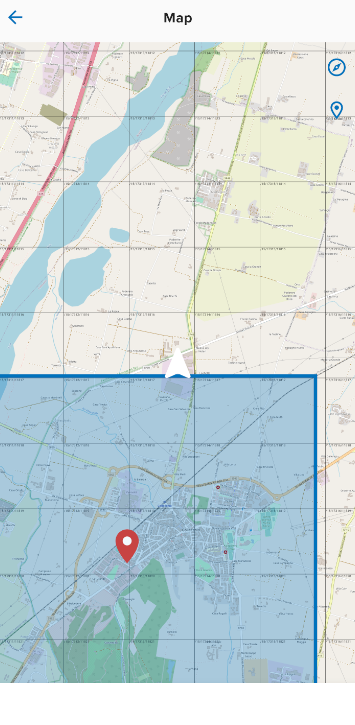
\includegraphics[width=0.4\textwidth]{Immagini/zoom_vicino.png}
    \caption{Zoom della mappa all'apertura}
    \label{fig:zoom_vicino}
\end{figure}

Questa scelta è stata motivata dall'ipotesi che, in un caso d'uso normale, l'utente non utilizzi questa mappa come navigatore e, pertanto, non dovrebbe aprirla quando si trova a grandi distanze dal luogo di lavoro. Si è ipotizzato che l'utente debba aprire la mappa solamente in prossimità del luogo di lavoro per comprendere la relazione tra la sua posizione e il luogo di lavoro, utilizzando la mappa come supporto per raggiungere il luogo dove registrare la propria presenza. Pertanto, si è ritenuto che fosse efficace per l'utente visualizzare la sua posizione e il luogo di lavoro più vicino al fine di orientarsi facilmente.

Durante la fase di progettazione dell'interfaccia grafica, si è valutato che la mappa dovesse fornire degli strumenti che agevolassero l'utente nel suo utilizzo. Per fare questo, è stata implementata una funzionalità di "follow-me", attivabile tramite un bottone sulla schermata della mappa. All'attivazione della funzionalità di "follow-me", la mappa scorre automaticamente, seguendo lo spostamento dell'utente, e rimane centrata sulla posizione dell'utente. Questa funzionalità agevola la navigazione dell'utente nello spazio che lo circonda, perché, nello spostamento per raggiungere il luogo di lavoro, non deve continuamente interagire con la mappa per vedere la sua posizione su di essa.

Inoltre, è stata considerata l'aggiunta di un bottone che permette all'utente di centrare la mappa sulla sua posizione corrente, in modo che anche se dovesse interagire con la mappa togliendo dal focus il marker con la sua posizione, non perda contezza di dove è la sua posizione, ma con un click la ritrovi immediatamente.



\chapter{Implementazione}
\label{cap4}

In questo capitolo verrà esplorata l'implementazione delle funzionalità chiave per il miglioramento della funzionalità di monitoraggio delle presenze di ZConnect. Nella Sezione 4.1, sarà analizzato l'algoritmo appositamente progettato per determinare la porzione di mappa da visualizzare quando l'utente apre la mappa, con l'obiettivo di fornire una chiara visualizzazione della posizione dell'utente e dell'area di lavoro più vicina. Verrà introdotto, nella Sezione 4.2, l'algoritmo utilizzato per calcolare la distanza tra la posizione dell'utente e il bordo più prossimo del geofence. Successivamente, nella Sezione 4.3, verrà esplorata l'implementazione della funzionalità ``follow-me", focalizzandosi su come questa caratteristica agevoli l'utente a raggiungere il luogo di lavoro preposto avendo il supporto della mappa. Infine, nella Sezione 4.4, verrà affrontato il tema della prevenzione della falsificazione della posizione nell'ambiente iOS di ZConnect, evidenziando le scelte implementative adottate.

\section{Determinare la porzione di mappa da visualizzare}
Un aspetto critico per il miglioramento della funzionalità di monitoraggio delle presenze di ZConnect, come visto nella Sezione \ref{Progettazione}, è quello di fornire all'utente, all'apertura della mappa, una visuale esaustiva della sua posizione e dell'area di lavoro a lui più vicina.

Per fare questo è stato necessario definire un algoritmo, chiamato zoomToUserAndGeoFence, a cui, passata la posizione dell'utente ed il geofence a lui più vicino, mostri la porzione di mappa corretta, che comprenda la posizione dell'utente ed il centro del geofence più vicino.
La determinazione del geofence più vicino all'utente verrà approfondita nella Sezione 4.2.

\begin{lstlisting}[
    basicstyle=\footnotesize, language = Java %or \small or \footnotesize etc.
]
void zoomToUserAndGeoFence(IGeoPoint geoPoint, GeoFenceWithDistance geoFence);
\end{lstlisting}

Come già analizzato, le versioni Android e iOS di ZConnect utilizzano librerie diverse per visualizzare la mappa. La versione Android di ZConnect utilizza la libreria Osmdroid.

La libreria Osmdroid tra i vari metodi e classi fornisce la classe BoundingBox \cite{BoundingBox}, che definisce una porzione di mappa tramite quattro coordinate geografiche: nord, sud, est ed ovest, modellate come float. Questa classe risulta quindi essenziale per poter definire la porzione di mappa da visualizzare. Di conseguenza per definire la porzione di mappa da visualizzare è stato imperativo definire i quattro vertici della BoundingBox.

Per fare questo, inizialmente è stato necessario calcolare il raggio della BoundingBox, ovvero il raggio della porzione di mappa da visualizzare. \'E stato scelto come raggio la distanza tra la posizione dell'utente ed il centro del geofence, il cui calcolo verrà illustrato in seguito, per avere la certezza che nella porzione di mappa scelta fosse sempre compresa la posizione dell'utente ed il centro del geofence a lui più vicino.

I vertici della BoundingBox sono però modellati come gradi di latitudine e longitudine, si è quindi reso necessario convertire la distanza, espressa in metri, in gradi di latitudine e longitudine. 
Per ottenere questo risultato sono state usate delle approssimazioni, in particolare si è considerato che $111111$ metri sono $1$ grado di latitudine e che $\frac{\text{distanza}}{ 111111 \cdot \cos{\text{\{latitudine\}}}} $ è un grado di longitudine.

Quindi ipotizzando che al metodo zoomToUserAndGeoFence siano passati i seguenti dati, che rappresentano le coordinate della posizione dell'utente e le coordinate del geofence:

\begin{lstlisting}[
    basicstyle=\footnotesize, language = Java %or \small or \footnotesize etc.
]
geoPoint.getLatitude = 44.87
geoPoint.getLongitude = 010.21

geoFence.getMaxLatitude = 44.86
geoFence.getMaxLongitude = 10.28
geoFence.getMinLatitude = 44.86
geoFence.getMinLongitude = 10.27

geoFence.getDistanceToCenter = 5154.18 metri
\end{lstlisting}

vengono calcolati i gradi di latitudine e longitudine della distanza tra la posizione dell'utente ed il centro del geofence con le approssimazioni precedentemente illustrate:

\[\begin{split}
    &\text{longitudeBoundingBoxRadious} = | \frac{5154.18}{111111} | = 0.046 \\
    &\text{latitudeBoundingBoxRadious} = | \frac{5151.18}{\cos{44.87 \cdot 111111}} | = 0.06
\end{split}\]

Dopo aver calcolato i gradi di latitudine e longitudine corrispondenti alla distanza tra l'utente ed il centro del geofence a lui più vicino sono stati determinati i vertici della BoundingBox trovando i punti più a Nord, Est, Sud e Ovest.
Per determinare questi punti è stato scelto come punto centrale della BoundingBox la posizione dell'utente, rendendo così necessario sommare e sottrarre opportunamente la latitudine e la longitudine della distanza tra la posizione dell'utente ed il centro del geofence con la latitudine e longitudine della posizione dell'utente.
Per determinare il punto più a Nord è stata sommata la latitudine della posizione dell'utente con la latitudine della distanza tra l'utente ed il centro del geofence. Per determinare il punto più a Est è stata sottratta la longitudine della distanza tra l'utente ed il centro del geofence alla longitudine della posizione dell'utente. Per determinare il punto più a sud è stata sottratta la latitudine della distanza tra l'utente ed il centro del geofence alla latitudine della posizione dell'utente. Infine per determinare il punto più ad ovest è stata sommata la longitudine della posizione dell'utente con la longitudine della distanza tra l'utente ed il centro del geofence.
Così facendo è stata determinata la porzione di mappa da mostrare.

Con i dati precedenti si otterrebbero i seguenti vertici:

\[\begin{split}
    &\text{Nord}: 44.87 + 0.06 = 44.93 \\
    &\text{Est}: 010.21 - 0.046 = 010.16 \\
    &\text{Sud}: 44.87 - 0.06 = 44.81 \\
    &\text{Ovest}: 010.21 + 0.046 = 010.26 \\
\end{split}\]

Nella versione iOS di ZConnect per definire la porzione di mappa da visualizzare è stata utilizzata la classe MKPolygon \cite{MKPolygon}, la quale permette di definire un poligono passando come argomenti del costruttore una lista di vertici modellati come latitudini e longitudini. \' E stato necessario anche per la versione iOS calcolare i quattro vertici del MKPolygon per determinare la porzione di mappa da visualizzare. Per fare questo sono stati eseguiti gli stessi passaggi illustrati in precedenza per la versione Android di ZConnect.

Con i dati di esempio precedente si ottiene la porzione di mappa in Figura \ref{fig:porzione_mappa}.

\begin{figure}[ht!]
    \centering
    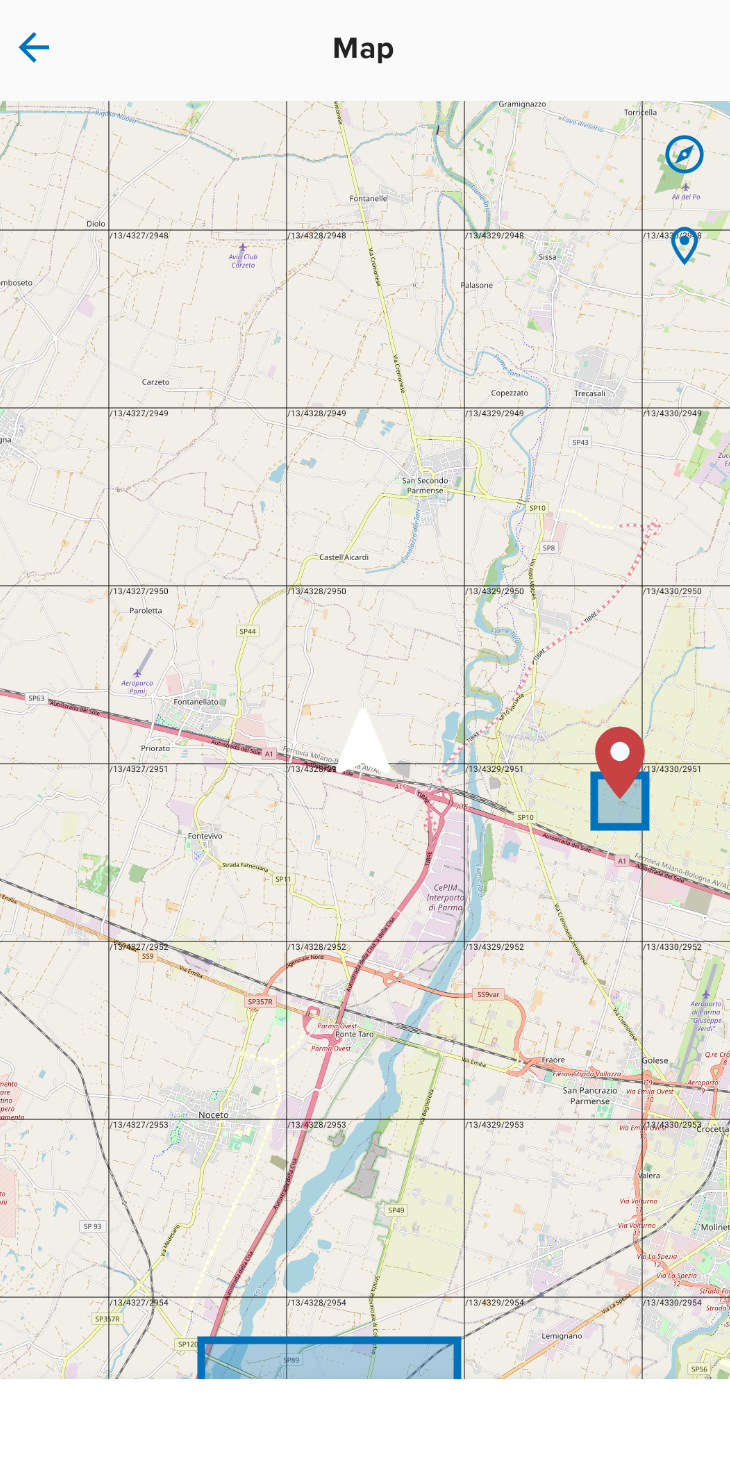
\includegraphics[width=0.4\textwidth]{Immagini/zoom_dati_esempio.png}
    \caption{Porzione di mappa ottenuta nella Sezione 4.1}
    \label{fig:porzione_mappa}
\end{figure}

\section{Distanza dal bordo del geofence}
Per determinare la porzione di mappa da mostrare è stato necessario stabilire quale fosse il luogo di lavoro più vicino all'utente nel momento in cui apre la mappa. Per stabilire quale luogo di lavoro fosse più vicino all'utente, dato che, come già visto, ad un utente è associata una lista di luoghi di lavoro, si è scelto di ordinare la lista dei luoghi di lavoro associata all'utente in base alla distanza tra il luogo di lavoro e l'utente, per poi scegliere il luogo di lavoro con distanza minore. In queste Sezione verrà trattato l'algoritmo per calcolare la distanza tra la posizione dell'utente ed un luogo di lavoro.

Come approfondito nella Sezione \ref{Analisi_sistema}, un area di lavoro è modellata come un istanza della classe GeoFence. Tutti i geofence utilizzati sono di tipo quadrato e sono definiti da quattro properties che servono ad identificare i vertici del quadrato, ovvero le latitudini e longitudini massime e minime. Inoltre ogni geofence ha associato il suo centro, modellato come un istanza della classe GeoPoint, che è una classe creata per rappresentare all'interno di ZConnect delle posizioni di punti sulla superficie terrestre, infatti ogni GeoPoint è identificato dalla sua latitudine e longitudine.

Date queste caratteristiche, per stabilire quale sia il geofence più vicino all'utente è necessario stabilire, per ogni geofence associato all'utente, la distanza tra la posizione dell'utente ed il bordo del geofence più prossimo. \'E fondamentale anche calcolare la distanza tra la posizione dell'utente ed il centro del geofence, poiché in caso di due o più geofence con distanza tra l'utente ed il bordo più prossimo uguale, viene considerato come geofence più vicino quello con distanza tra la posizione dell'utente ed il centro minore.

\subsection{Determinare il bordo più vicino}
Per calcolare la distanza tra la posizione dell'utente ed il bordo del geofence più prossimo all'utente è necessario prima stabilire qual'è il bordo del geofence più vicino all'utente, evitando così di calcolare la distanza tra la posizione dell'utente ed ogni bordo del geofence per poi selezionare la distanza minore.

Nella classe GeoFence è stato creato un metodo, calculateDistanceToBorder, che prende come argomento un GeoPoint e restituisce la distanza tra il punto passato come argomento e il bordo più vicino al GeoFence stesso. Per determinare quale sia il bordo del geofence più vicino alla posizione passata sono stati inizialmente identificati i quattro vertici del geofence, è stato possibile farlo perchè il geofence ha come properties le latitudini e longitudini massime e minime. Quindi i vertici del geofence sono modellati come GeoPoint risultanti dal prodotto cartesiano tra le latitudini e le longitudini del geofence.
Ad esempio se le properties del geofence sono i seguenti:
\begin{lstlisting}[
    basicstyle=\footnotesize, language = Java %or \small or \footnotesize etc.
]
maxLatitude = 44.77
maxLongitude = 10.23
minLatitude = 44.72
minLongitude = 10.17
\end{lstlisting}

i vertici dei geofence verranno composti in questo modo:

\begin{lstlisting}[
    basicstyle=\footnotesize, language = Java %or \small or \footnotesize etc.
]
GeoPoint top_right_vertex = new GeoPoint(maxLatitude, maxLongitude);
GeoPoint top_left_vertex = new GeoPoint(maxLatitude, minLongitude);
GeoPoint bottom_left_vertex = new GeoPoint(minLatitude, minLongitude);
GeoPoint bottom_right_vertex = new GeoPoint(minLatitude, maxLongitude);
\end{lstlisting}

Dopo aver identificato i vertici del geofence, si è deciso, immaginando di posizionare il geofence su un piano cartesiano, che rappresenta la superficie terrestre, di dividere lo spazio in settori; proiettando verso più e meno infinito le latitudini e longitudini massime e minime del geofence. Così facendo si vengono a creare nove settori. Come si può vedere nella tabella \ref{tab:settori} i settori sono stati numerati sequenzialmente, partendo dal settore in alto a sinistra. Seguendo questa numerazione il settore cinque è quello che rappresenta l'area del geofence.

\begin{table}[ht!]
    \centering
    \begin{tabular}{c|c|c}
       1 & 2 & 3 \\
       \hline
       4 & 5 & 6 \\
    \hline
       7 & 8 & 9
    \end{tabular}
    \caption{Divisione dello spazio in settori}
    \label{tab:settori}
\end{table}

Una volta identificati questi settori, confrontando la latitudine e la longitudine della posizione dell'utente con la latitudine e longitudine dei vertici del geofence, è possibile stabilire in che quadrante è posizionato l'utente.
Ad esempio se la posizione dell'utente, che è passata come argomento al metodo calculateDistanceToBorder, ha la seguente latitudine e longitudine:
\begin{lstlisting}[
    basicstyle=\footnotesize, language = Java %or \small or \footnotesize etc.
]
point_latitude = 37.42
point_longitude = -122.08
\end{lstlisting}

Confrontando la latitudine e la longitudine della posizione dell'utente con le latitudini e longitudini minime e massime del geofence, si stabilisce che la posizione dell'utente cade nel settimo settore, in quanto la latitudine della posizione dell'utente è minore uguale della latitudine minima del geofence e la longitudine della posizione dell'utente è minore uguale della longitudine minima del geofence.

Una volta identificato qual'è il settore in cui è contenuta la posizione dell'utente si è stabilito anche qual'è il bordo più vicino all'utente, in quanto è sempre il bordo che fa parte del settore identificato.
Nei casi in cui la posizione dell'utente sia contenuta nei quadranti 1, 3, 7 e 9, non viene identificato il bordo del geofence, ma viene identificato un vertice, in quanto, per qualsiasi posizione all'interno di questi quadranti, la distanza minima tra quella posizione ed il geofence sarà sempre la distanza tra quella posizione ed il vertice contenuto nel quadrante identificato. 
Nell'esempio precedente quindi viene identificato come bordo più vicino il vertice bottom\_left\_vertex.

\subsection{Calcolo della distanza dal bordo}
Grazie all'algoritmo precedentemente illustrato è stato possibile identificare quale fosse il bordo del geofence più vicino all'utente. Avendo identificato il bordo più vicino, modellato tramite i due vertici che lo compongono, che a loro volta sono modellati tramite istanze della classe GeoPoint, è stato possibile calcolare la distanza minima tra la posizione dell'utente ed il bordo identificato come quello più vicino all'utente.

Come visto in precedenza, si può identificare come bordo più vicino un segmento o un punto. Nel caso in cui venga identificato un punto è necessario calcolare la distanza tra due punti, la posizione dell'utente e il vertice del geofence identificato come quello più vicino all'utente. Per raggiungere questo obiettivo è stato implementato un metodo nella classe GeoPoint, getHaversineDistance:
\begin{lstlisting}[
    basicstyle=\footnotesize, language = Java %or \small or \footnotesize etc.
]
/**
* Computes the minimum distance between current geopoint and a second 
* geopont using the Haversione Formula
* @param from The geopoint from which to compute distance
* @return The distance
*/
double getHaversineDistance(IGeoPoint from);
\end{lstlisting}

che permette di calcolare la distanza tra la posizione dell'utente, modellata tramite un'istanza della classe GeoPoint, ed una seconda posizione, passata come argomento del metodo stesso, utilizzando la formula di Haversine. La formula di Haversine determina la distanza tra due punti su una sfera, date le loro longitudini e latitudini.
Viene riportata di seguito la formula di Haversine, dove $\phi$ è la latitudine, $\lambda$ è la longitudine e $R$ è il raggio della terra:

\begin{align*}
a & = \sin^2\left(\frac{\phi_2 - \phi_1}{2}\right) + \cos\phi_1 \cdot \cos\phi_2 \cdot \sin^2\left(\frac{\lambda_2 - \lambda_1}{2}\right) \\
c & = 2 \cdot \mathrm{atan2}\left(\sqrt{a}, \sqrt{1-a}\right) \\
d & = R \cdot c
\end{align*}

Invece, nel caso in cui venga identificato un segmento è necessario calcolare la distanza minima tra un punto ed un segmento. Per fare questo è stato implementato un altro metodo nella classe GeoPoint, getMinimumDistancePointLine:

\begin{lstlisting}[
    basicstyle=\footnotesize, language = Java %or \small or \footnotesize etc.
]
/**
* Computer the distance bewteen two given geopoint and a third geopoint
*
* @param vertex1
* @param vertex2
* @return
*/
double getMinimumDistancePointLine(IGeoPoint vertex1, IGeoPoint vertex2);
\end{lstlisting}

che permette di calcolare la distanza tra la posizione, modellata tramite l'istanza della classe GeoPoint, ed un segmento, modellato tramite i suoi due vertici, passati come argomento al metodo stesso.
Innanzitutto è stato calcolato l'angolo di Bearing assoluto dei due segmenti formati dai vertici del bordo più vicino e la posizione dell'utente. L'angolo di Bearing è l'angolo formato tra il segmento ed il nord magnetico.
Considerando la posizione dell'utente come punto A ed i vertici del segmento come punti B e C, il calcolo dell'angolo di Bearing è il seguente, dove $\phi$ è la latitudine, $\lambda$ è la longitudine e $R$ è il raggio della terra:

\begin{align*}
\text{bearingAC} & = \mathrm{atan2}\left( \sin(\lambda_C - \lambda_A) \cdot \cos(\phi_2), \cos(\phi_1) \cdot \sin(\phi_2) - \sin(\phi_1) \cdot \cos(\phi_2) \cdot \cos(\phi_C - \phi_A) \right) \\
\text{bearingAB} & = \mathrm{atan2}\left( \sin(\lambda_B - \lambda_A) \cdot \cos(\phi_2), \cos(\phi_1) \cdot \sin(\phi_2) - \sin(\phi_1) \cdot \cos(\phi_2) \cdot \cos(\phi_B - \phi_A) \right)
\end{align*}

Gli angoli di Bearing ottenuti sono stati normalizzati, in modo da ottenere valori compresi tra 0 e 360.
Successivamente è stata calcolata la distanza tra il punto A ed il punto C utilizzando la formula di Haversine, precedentemente illustrata.
Infine è stata calcolata la cross-track distance, ovvero la distanza tra un punto ed un segmento su una sfera, distanza chiamata great circle path.
La formula per calcolare la cross-track distance è la seguente:

\begin{align*}
d_{xt} = \sin^{-1}\left( \sin(\delta_{13}) \cdot \sin(\theta_{13} - \theta_{12}) \right) \cdot R
\end{align*}

dove:
\begin{itemize}
    \item $\delta_{13}$ è la distanza tra il punto di partenza ed il terzo punto. Nell'esempio precedente è la distanza tra A e C
    \item $\theta_{13}$ è l'angolo di Bearing tra il punto di partenza ed il terzo punto. Nell'esempio precedente è l'angolo di Bearing del segmento AC.
    \item $\theta_{12}$ è l'angolo di Bearing tra il punto di partenza ed il secondo punto. Nell'esempio precedente è l'angolo di Bearing del segmento AB.
    \item $R$ è il raggio della terra.
\end{itemize}

Grazie a questo algoritmo viene calcolata la distanza tra la posizione dell'utente ed il bordo del geofence che permette di selezionare il geofence più vicino all'utente nel momento in cui apre la mappa.

\section{Follow-me}
Per migliorare la funzionalità di monitoraggio delle presenze di ZConnect in questo lavoro di tesi è stato deciso di implementare la funzionalità del ``follow-me", come approfondito nella Sezione \ref{Progettazione}. Questa funzionalità facilita l'utente nel raggiungimento dell'area di lavoro poiché, una volta attivata, il marker che rappresenta la posizione dell'utente rimane al centro della schermata della mappa durante gli spostamenti dell'utente.

Anche in questo caso, a causa del duplice sviluppo di ZConnect per Android l'implementazione di questa funzionalità cambia notevolmente tra i due sistemi operativi.

Come già detto la versione Android di ZConnect utilizza la libreria Osmdroid \cite{OpenStreetMapWiki} per la visualizzazione e l'interazione con la mappa. La libreria Osmdroid fornisce una classe, MyLocationNewOverlay \cite{MyLocationNewOverlay}, che permette di rappresentare la posizione del device sulla mappa tramite un marker. La classe MyLocationNewOverlay ha associato un LocationProvider \cite{LocationProvider}, passato come argomento nel costruttore, grazie al quale è in grado di conoscere la posizione del device e reagire agli spostamenti, ridisegnando il marker sulla mappa. Inoltre la classe MyLocationNewOverlay espone i metodi enableFollowLocation e disableFollowLocation, i quali permettono di abilitare la funzionalità ``follow-me" che permette di centrare la mappa sulla posizione corrente del MyLocationNewOverlay e automaticamente spostarla quando viene rilevato un cambio di posizione, in modo da far rimanere sempre al centro della mappa il marker che rappresenta la posizione del dispositivo.

Quindi per implementare la funzionalità di ``follow-me" nella versione Android è bastato utilizzare come marker per la posizione dell'utente un istanza della classe MyLocationNewOverlay ed utilizzare i suoi metodi per attivare e disattivare la funzionalità, la quale viene poi gestita in automatico dalla libreria Osmdroid.

A differenza di Android, la versione iOS di ZConnect utilizza la libreria MapKit \cite{MapKitDoc} che è fornita direttamente da Apple.
La libreria MapKit fornisce la classe MKMapView usata per mostrare ed interagire con la mappa \cite{MKMapView}. La libreria MKMapView implementa dei metodi per mostrare e manipolare dei contenuti sulla mappa. Per mostrare la posizione del device sulla mappa è stato utilizzato il metodo showUserLocation della classe MKMapView. Attivando questa funzione viene visualizzato sulla mappa un marker blu in corrispondenza della posizione del device. Il marker reagisce anche allo spostamento del device ridisegnandosi in corrispondenza della nuova posizione rilevata.

La libreria MapKit non fornisce, a differenza di Osmdroid, la funzionalità ``follow-me" integrata nella classe che rappresenta il marker dell'utente. Quindi per implementare la funzionalità di ``follow-me" è stata usata la classe MKMapCamera \cite{MKMapCamera} fornita anch'essa dalla libreria MKMapKit. Un'istanza di questa classe definisce un punto di vista virtuale sopra la superficie della mappa e influenza il modo in cui MapKit presenta la mappa all'utente.

La classe MKMapView fornisce una funzione di call-back che viene chiamata dal sistema operativo quando la posizione del device cambia, in questa funzione viene controllato se l'utente ha attivato funzionalità di ``follow-me", se è attiva viene settata la property centerCoordinate, della classe MKMapCamera, con le coordinate prese dalla posizione dell'utente, che la classe MKMapView salva nella variabile userLocation. Dopo aver settato le coordinate del centro della mappa, tramite la funzione setCamera della classe MKMapView viene animata la mappa per essere centrata sulla nuova posizione dell'utente.

Così facendo è stata implementata la funzionalità di ``follow-me" in iOS, agevolando anche gli utenti della versione iOS di ZConnect nel raggiungimento dell'area di lavoro.

\section{Fake position iOS}
Nel capitolo di Analisi si era identificato come caratteristica dell'applicazione la prevenzione di possibili falsificazioni della posizione del dispositivo da parte dell'utente, in modo da evitare che l'utente possa registrare la propria presenza sul posto di lavoro anche quando non è fisicamente lì.
Questo controllo sulla falsificazione della posizione dell'utente nella versione iOS di ZConnect non era stato implementato prima di questo lavoro di tesi, a differenza della versione Android di ZConnect che controllava anche prima di questo lavoro di tesi la veridicità della posizione dell'utente.

Quindi è stato necessario implementare un controllo sulla eventuale falsificazione della posizione dell'utente nella versione iOS di ZConnect.

La classe che si occupa di implementare la classe che in iOS si occupa di rilevalre la posizione dell'utente è LocationManager. La classe che in iOS si occupa di rilevare la posizione del device è CLLocationManager. Il CLLocationManager è il luogo centrale per gestire i comportamenti legati alla posizione dell'applicazione. Si può utilizzare un oggetto location-manager per configurare, avviare e interrompere i servizi di localizzazione \cite{CLLocationManager}.

Nella classe LocationManager è stato creato un metodo, isMockLocation, per identificare se la posizione rilevata dal CLLocationManager è fittizia oppure deriva dalla vera posizione del device. Per raggiungere questo obiettivo sono stati usati i metodi isSimulatedBySoftware e isProducedByAccessory della classe CLLocationSourceInformation. La classe CLLocationSourceInformation contiene informazioni sulla fonte che fornisce un'istanza di CLLocation \cite{CLLocationSourceInformation}. Un oggetto CLLocation contiene la posizione geografica e l'altitudine di un dispositivo, insieme a valori che indicano l'accuratezza di tali misurazioni e il momento in cui sono state raccolte \cite{CLLocation}.
Il metodo isSimulatedBySoftware restituisce un valore booleano che indica se la posizione rilevate è stata generata da un software come Xcode, mentre il metodo isProducedByAccessory restituisce un valore booleano che indica se la posizione è stata generata da un accessorio esterno.

Il metodo isMockLocation, implementato nella classe LocationManager, controlla i risultati dei metodi isSimulatedBySoftware e isProducedByAccessory. Se uno dei due risultati è vero allora la posizione rilevata dal CLLocationManager è stata falsificata dall'utente.

Ora, per verificare se una posizione è stata falsificata, è necessario invocare il metodo isMockLocation dall'istanza della classe LocationManager, utilizzata per ottenere la posizione del dispositivo. Questo metodo esegue un controllo per determinare se la posizione ricevuta dal CLLocationManager è di natura simulata o rappresenta effettivamente la reale posizione del dispositivo.

\chapter{Testing}
\label{cap5}

Per poter rilasciare sul mercato la nuova versione di ZConnect creata dopo le modifiche effettuate nella Sezione di Implementazione di questa tesi, Zucchetti S.P.A. ha affidato il compito di testare la migliorata funzionalità di monitoraggio delle presenze ad un team specifico di tester. Durante questo lavoro di tesi è stato seguito anche il team di tester, che tramite dei test funzionali ha validato la nuova versione di ZConnect. Le metodologie di test ed i risultati prodotti saranno rispettivamente descritti nelle Sezioni 5.1 e 5.2.

\section{Metodologia di test}
Durante questo lavoro di tesi, ho seguito anche il team di tester durante l'esecuzione dei test per poter rilasciare sul mercato la nuova versione di ZConnect. Il team di tester ha eseguito dei test funzionali. I test funzionali vengono utilizzati per individuare le discrepanze tra le specifiche e l'effettiva implementazione dei sistemi software \cite{TestFunzionali}. Tutti i test riportati di seguito sono stati eseguiti sia sulla versione Android che sulla versione iOS di ZConnect.

Inoltre, per far fronte al problema della frammentazione hardware e software tipico delle applicazioni per dispositivi mobili \cite{AndroidFragmentation}, tutti i test sono stati effettuati su dispositivi fisici con la versione minima e massima dei sistemi operativi per cui è sviluppata l'applicazione. In altre parole, è stato utilizzato un dispositivo Android con installata la versione 7 di Android e un dispositivo con installata la versione 13 di Android. Per iOS, è stato utilizzato un dispositivo fisico con installata la versione 14 di iOS e un dispositivo con installata la versione 16 di iOS. L'applicazione è stata testata anche su un tablet Android, poiché ZConnect è disponibile anche per tablet.

Il primo test funzionale eseguito è stato quello di apertura della mappa con un utente che ha associato numerose aree di lavoro per verificare che sulla mappa fossero presenti tutte le aree di lavoro, modellate tramite geofence, al cui centro fosse visibile un marker rosso che identifica il centro del geofence e che fosse visibile la posizione dell'utente identificata con un marker blu.

Successivamente è stato provato se cambiando la posizione dell'emulatore il marker dell'utente reagisse al cambio di posizione spostandosi a sua volta. Sono anche stati provati il pulsante per centrare la mappa sulla posizione dell'utente ed il pulsante per il ``follow-me", controllando che all'attivazione e alla disattivazione del ``follow-me" il pulsante cambi colore, in modo da dare un feedback adeguato all'utente. Con la funzionalità ``follow-me" attiva è stato provato a mettere l'app in background ed a riportala in foreground per verificare che la funzionalità rimanesse attiva. Infine è stato provato ad impostare, la modalità scura dell'app per vedere che i nuovi elementi grafici aggiunti alla mappa reagissero al cambiamento cambiando a loro volta colore. 


\begin{figure}[ht!]
    \begin{subfigure}{0.4\textwidth}
        \centering
        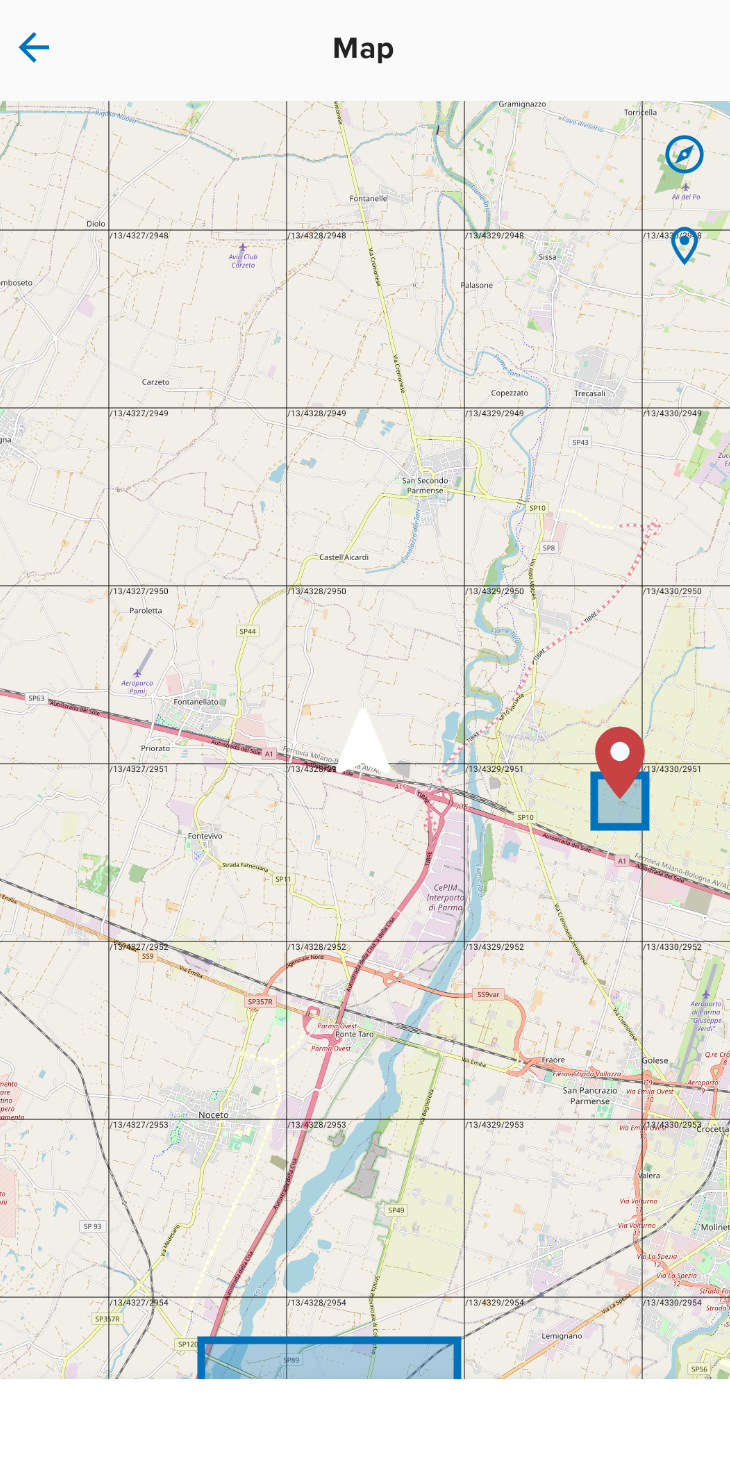
\includegraphics[width=\linewidth]{Immagini/zoom_dati_esempio.png}
        \caption{``follow-me" disattivo}
        \label{fig:vecchia_posizione_esterna_Android_2}
    \end{subfigure}
    \hspace{1cm} % Spazio orizzontale tra le immagini
    \begin{subfigure}{0.4\textwidth}
        \centering
        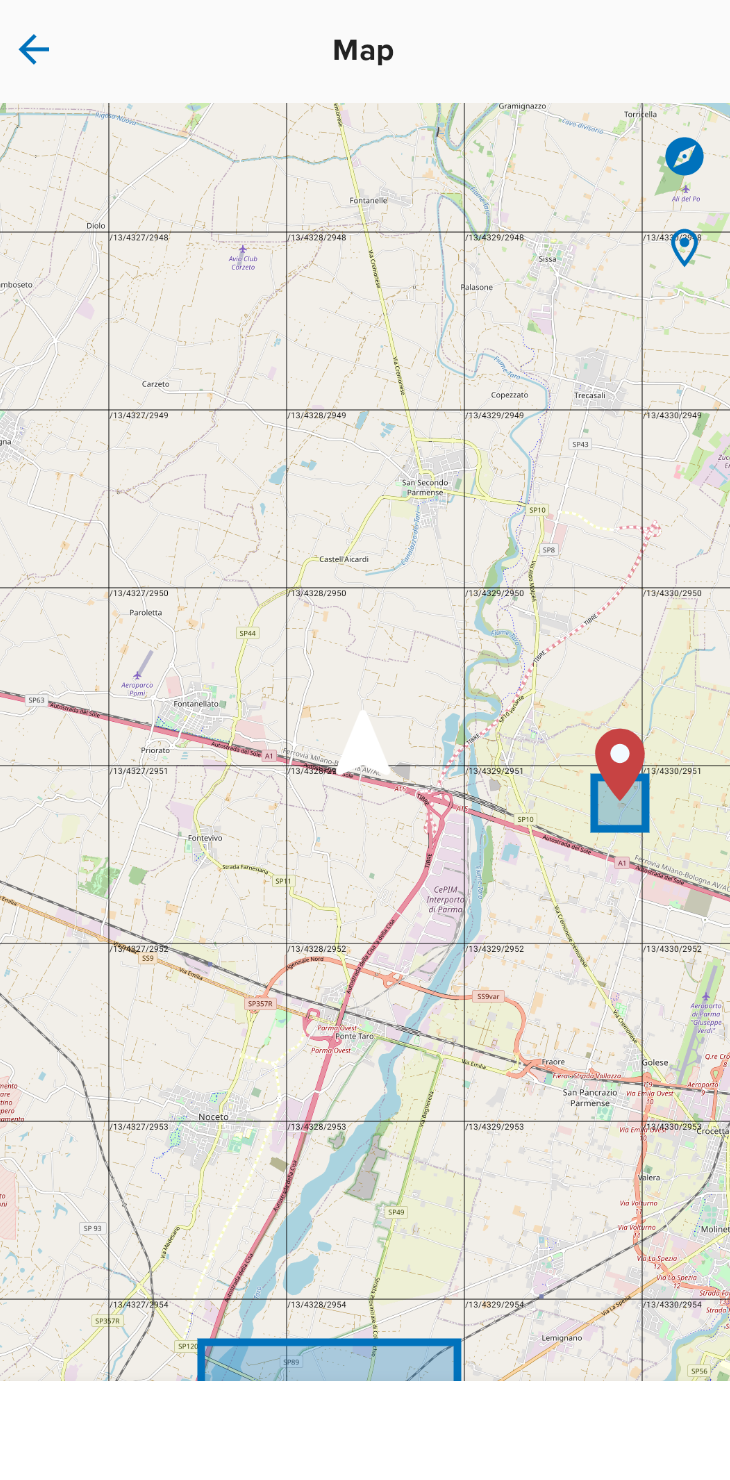
\includegraphics[width=\linewidth]{Immagini/follow_me_attivo.png}
        \caption{``follow-me" attivo}
        \label{fig:vecchia_posizione_interna_Android_2}
    \end{subfigure}
    \caption{Cambio del fill del bottone per attivare la funzione ``follow-me"}
    \label{fig:vecchia_mappa_android_3}
\end{figure}

Infine sono stati eseguiti dei test di non regressione. I test di non regressione vengono impiegati per verificare che le modifiche apportate al codice, gli aggiornamenti o le correzioni di errori non generino problemi alle funzionalità preesistenti dell'applicazione o del software, evitando nel contempo eventuali instabilità non correlate alle caratteristiche specifiche.
\' E stato provato ad effettuare una timbratura all'esterno ed all'interno di un area di lavoro associata all'utente, per verificare che nel caso della timbratura effettuata all'esterno dell'area di lavoro associata all'utente che questa venisse rifiutata, mentre nel caso di timbratura effettuata all'interno dell'area di lavoro associata all'utente che questa venisse accettata.
Infine è stato provata la visualizzazione della mappa sulla schermata delle timbrature passate, per testare che fosse ancora navigabile e che il luogo di lavoro dove è stata eseguita la timbratura fosse ancora visibile, modellato come un geofence.

\section{Risultati dei test}
I test funzionali illustrati nella Sezione 5.1 hanno prodotto per lo più risultati positivi.
\'E stato riscontrato un solo problema, che nella versione Android di ZConnect se viene attivata la funzionalità di ``follow-me" e successivamente, con la funzionalità attiva, l'applicazione viene messa in background e riportata in foreground, la funzionalità di ``follow-me" risulta non attiva. 

Grazie all'esecuzione di questi test funzionali è stato possibile individuare delle problematiche la cui risoluzione ha portato al rilascio di una versione di ZConnect funzionante e conforme alle specifiche descritte nella fase di analisi di questa tesi.

\chapter{Conclusioni}
\label{cap6}

Con il presente lavoro di tesi sono stati ottenuti dei risultati, che verranno delineati nella Sezione 6.1, esaminandoli criticamente e mettendo in evidenza le realizzazioni e le scoperte emerse durante l'analisi, lo sviluppo e la valutazione delle soluzioni proposte. La Sezione 6.2 fornirà uno sguardo approfondito sui limiti di questo lavoro e sulle sfide incontrate durante il corso di questo progetto. La Sezione 6.3 analizzerà le prospettive future del presente lavoro, suggerendo vie potenziali per ulteriori sviluppi. Questa Sezione non solo proietterà lo sguardo oltre la conclusione di questo progetto, ma fornirà anche una base per ulteriori contributi e iterazioni sulle soluzioni proposte.

\section{Risultati ottenuti}
Grazie al lavoro di analisi, progettazione, sviluppo e test, questa tesi ha portato alla creazione di una nuova versione dell'applicazione ZConnect, migliorata secondo le richieste dell'Azienda X nella sua funzionalità di monitoraggio delle presenze. La collaborazione con il team di sviluppo di ZConnect e il team di test ha permesso il rilascio della versione migliorata, attualmente disponibile sugli store di Android ed iOS, con un ampio utilizzo da parte di centinaia di migliaia di utenti.

La recente evoluzione della funzionalità di monitoraggio delle presenze è stata guidata dalle esigenze specifiche dell'Azienda X, la quale ha espresso piena soddisfazione per il lavoro svolto. I miglioramenti apportati riguardano principalmente la mappa di ZConnect, ora progettata in modo da rendere chiare all'utente sia la propria posizione che quella dell'area di lavoro più vicina. Per fornire un maggior supporto all'utente nel raggiungere l'area di lavoro, è stata migliorata l'usabilità della mappa e introdotta la funzionalità "follow-me", ideata per guidare l'utente in modo più intuitivo verso il luogo di lavoro.

\section{Limiti del sistema}
L'analisi dei risultati di questo lavoro ha rivelato alcune limitazioni.
In primo luogo, la mancanza di test di usabilità con gli utenti rappresenta una limitazione significativa. Questi test avrebbero fornito un feedback diretto sull'efficacia delle modifiche apportate al sistema di monitoraggio delle timbrature, valutando se le soluzioni implementate hanno effettivamente risolto i problemi dei dipendenti dell'Azienda X, senza introdurne di nuovi.

Una seconda limitazione è emersa dalla mancanza di test reali di utilizzo da parte del team di test. La verifica statica su dispositivi fisici non ha coperto l'aspetto dinamico dello spostamento dell'utente sulla mappa, trascurando l'efficacia della funzionalità "follow-me". La correttezza e l'utilità di questa caratteristica non sono state completamente validate, rappresentando un'area di incertezza.

Infine, la struttura stessa di ZConnect rappresenta un limite, poiché, come già visto, è sviluppata sia per Android che per iOS, duplicando le basi di codice. I problemi affrontati, e risolti, da questo lavoro di tesi avrebbero potuto essere gestiti più efficientemente da un'applicazione ibrida. Questo avrebbe potenzialmente ridotto i tempi di sviluppo e semplificato la gestione complessiva del software, in quanto un'app ibrida consente di scrivere le funzionalità dell'app in un'unica base di codice \cite{AppNative}.  

\section{Miglioramenti futuri}
L'analisi dei risultati di questo lavoro di tesi ha evidenziato potenziali miglioramenti della funzionalità di monitoraggio delle presenze di ZConnect.

In primo luogo, si potrebbe implementare l'inserimento di etichette esplicative al momento della pressione del marker rappresentante il centro del luogo di lavoro. Questa caratteristica aggiuntiva consentirebbe agli utenti di ottenere informazioni chiare e dettagliate sul luogo di lavoro selezionato.

In secondo luogo, considerando che un utente potrebbe avere numerose aree di lavoro associate, sarebbe utile consentire la ricerca di un luogo di lavoro specifico in base al suo nome. Tale funzionalità permetterebbe all'utente di posizionare la mappa direttamente sul luogo di lavoro desiderato, semplificando l'utilizzo della mappa.

Infine, un ulteriore miglioramento potrebbe consistere nell'introduzione di un sistema di navigazione. Una volta selezionato un luogo di lavoro, questa funzione consentirebbe all'utente di visualizzare sulla mappa il percorso ottimale per raggiungere la destinazione desiderata. Questo sistema di navigazione potrebbe notevolmente facilitare gli spostamenti degli utenti verso le varie sedi di lavoro associate, migliorando complessivamente l'esperienza di utilizzo della funzionalità di monitoraggio delle timbrature di ZConnect.

%
%			BIBLIOGRAFIA
%
\begin{thebibliography}{00}
\bibitem{GeoFence}
\url{https://learn.microsoft.com/en-us/dynamics365/field-service/mobile-powerapp-geofence}

\bibitem{OpenStreetMapWiki}
\url{https://it.wikipedia.org/wiki/OpenStreetMap}

\bibitem{MapKitDoc}
\url{https://developer.apple.com/documentation/mapkit/}
%
\bibitem{Android}
\url{https://www.android.com}
%
\bibitem{iOS}
\url{https://developer.apple.com/documentation/}
%
\bibitem{Kotlin}
\url{https://kotlinlang.org/docs/home.html}
%
\bibitem{Java}
\url{https://docs.oracle.com/en/java/}
%
\bibitem{Swift}
\url{https://www.swift.org/documentation/}

\bibitem{BoundingBox}
\url{https://osmdroid.github.io/osmdroid/javadocs/osmdroid-android/debug/index.html?org/osmdroid/util/BoundingBox.html}

\bibitem{MKPolygon}
\url{https://developer.apple.com/documentation/mapkit/mkpolygon}

\bibitem{MyLocationNewOverlay}
\url{https://osmdroid.github.io/osmdroid/javadocAll/org/osmdroid/views/overlay/mylocation/MyLocationNewOverlay.html}

\bibitem{LocationProvider}
\url{https://developer.android.com/reference/android/location/LocationProvider}

\bibitem{MKMapView}
\url{https://developer.apple.com/documentation/mapkit/mkmapview}

\bibitem{MKMapCamera}
\url{https://developer.apple.com/documentation/mapkit/mkmapcamera}

\bibitem{CLLocationManager}
\url{https://developer.apple.com/documentation/corelocation/cllocationmanager}

\bibitem{CLLocationSourceInformation}
\url{https://developer.apple.com/documentation/corelocation/cllocationsourceinformation}

\bibitem{CLLocation}
\url{https://developer.apple.com/documentation/corelocation/cllocation}

\bibitem{Fragment}
\url{https://developer.android.com/guide/fragments}

\bibitem{ViewController}
\url{https://developer.apple.com/documentation/uikit/uiviewcontroller}

\bibitem{TestFunzionali}
A. A. Omar and F. A. Mohammed. 1991. A survey of software functional testing methods. SIGSOFT Softw. Eng. Notes 16, 2 (April 1991), 75–82.
\url{https://dl.acm.org/doi/abs/10.1145/122538.122551}

\bibitem{AndroidFragmentation}
D. Han, C. Zhang, X. Fan, A. Hindle, K. Wong and E. Stroulia, "Understanding Android Fragmentation with Topic Analysis of Vendor-Specific Bugs," 2012 19th Working Conference on Reverse Engineering, Kingston, ON, Canada, 2012, pp. 83-92, doi: 10.1109/WCRE.2012.18.
\url{https://ieeexplore.ieee.org/document/6385104}

\bibitem{AppNative}
\url{https://aws.amazon.com/it/compare/the-difference-between-web-apps-native-apps-and-hybrid-apps/}
\end{thebibliography}
% 
\end{document}